\chapter{Performance Analysis of Bandwidth Aggregation Systems}\label{chap:aggregation}

In 2015, mobile networks carried more than 40 exabytes of traffic, which is expected to increase 8-fold towards 2020 \cite{cisco2016mobile}.
To handle the growth and to reduce the load on mobile networks, offloading to WiFi has come to the center of industry thinking \cite{wba2011wifi}.
%Mobile offload exceeded cellular traffic for the first time in 2015.
%Accoring to \cite{cisco2016mobile}, 51\% of total mobile data traffic was offloaded onto the fixed network through WiFi or femtocell.

In contrast to strict offloading, in which the Internet access link is switched completely, e.g., from cellular to WiFi, current concepts such as BeWifi\footnote{\url{http://www.tid.es/research/areas/bewifi}} also consider multiple connections to the Internet, thereby sharing and aggregating available backhaul access link capacities. The question is which sharing policy to apply for which system characteristics. In the case of BeWifi, which considers access link sharing among neighboring users, each user should only share its access link when having spare capacity in order to avoid negatively affecting his own Internet connections. Therefore, two thresholds were introduced, i) a support threshold until which utilization a user will offer bandwidth to other users, and ii) an offloading threshold indicating from which utilization a user can offload to supporting neighbors.
It is hard and non-intuitive to determine the threshold settings for fair and effective operation of a bandwidth sharing system.
In this work a partial bandwidth sharing environment with offloading policy is investigated using an analytic model.
A direct application of the model is the aggregation of backhaul bandwidth by connecting neighboring access links.
%Further applications are the aggregation of bandwidth of multihomed connections or upstreaming of mobile data via.
%Increasing the capacity of mobile access links helps managing the increasing amount of mobile data traffic.

We develop a Markov model to analyze the bandwidth aggregation potential of neighboring access links.
The Markov model is limited to two access links, which limits its applicability.
It was shown in pilot studies that the technology's only limitation is the actual WiFi bandwidth available.
In urban environments there are far more than two access links available.
As shown in \cite{sapiezynski2015tracking}, an average of 25 WiFi access points are visible in every scan in densely-populated areas.
In this case an assessment with the model previously proposed by the authors is not possible, since it is limited to two access links.
An extension of the Markov model to m dimensions would require solving an equation system with $n^m$ equations, which is computationally too complex.
We extend the Markov model to be applicable for two and more links using a fixed point approximation.
This allows us to reduce the n-dimensional Markov chain to evaluate the steady state probabilities efficiently.

%A highly loaded link can benefit from offloading to cooperating systems, receiving considerably more bandwidth than its own capacity.
%We provide analytic and simulative results for the received bandwidth and the bandwidth gain for each access link.
%As reference system we consider partitioned access links.

The contribution of this chapter is three-fold.
First, the approximation using fixed point iteration can be used to seamlessly evaluate the performance of systems between partitioning and complete sharing dependent on the threshold settings.
Second, by considering an outer and an inner composite system we are able to apply the method to the case of heterogeneous load, which is crucial to assess the full potential of the approach.
Bandwidth sharing systems are designed to increase the throughput of systems that are currently overloaded by using spare bandwidth of underutilized links.
In such situations the load on the links is highly heterogeneous.
Our results show that an overloaded system can greatly benefit, by receiving multiples of its own capacity, from spare bandwidth of underutilized cooperating systems.
Third, we evaluate the robustness of the mechanism against free riders by prioritizing links and find that altruistic users may only lose slightly more bandwidth than in normal operation.
This is important, since a bandwidth sharing system that is running an inefficient offloading policy may be exploited by free riders, which are users that claim spare bandwidth by offloading traffic, but do not share any of their own bandwidth.
%We find that with the considered considered threshold settings the received bandwidth can be up to 2\% lower than the baseline in partitioned operation.
%This is compensated by the fact that an overloaded system can highly benefit, by receiving multiples of its own capacity, from spare bandwidth of underutilized cooperating systems, especially if the number of cooperating systems is high.

The content of this chapter is mainly taken from~\cite{burger2016phycom,burger2017im}.
Its remainder is structured as follows.
\refsec{sec:aggregation:background} summarizes offloading and bandwidth sharing systems and technologies.
In \refsec{sec:aggregation:model}, the model of a bandwidth aggregation system is described in detail and results of the performance evaluation are reported. In \refsec{sec:aggregation:imbalanced} the model is extended to consider imbalanced systems loads, while this chapter is concluded with lessons learned in \refsec{sec:aggregation:lessonslearned}.

\section{Background and Related Work}\label{sec:p2p:background}

This section describes background of this chapter and presents related work. We start with an overview on measurement studies of live BitTorrent networks and show different approaches to reduce inter-ISP traffic discussed in the ALTO working group of the IETF. Finally, we introduce studies that infer the inter-AS relations based on BGP routing information.
We briefly describe the structure of the YouTube video CDN and give a short introduction in the principles of crowdsourcing.
Further, we summarize related work in the field of distributed active measurements of CDNs as well as work related to crowdsourcing aided network measurements.

\subsection{Measurements and Models of Live BitTorrent Networks}

BitTorrent is a peer-to-peer file-sharing protocol, which is based on multi-source downloads between the users. All the users, i.e., \textit{peers}, sharing the same file belong to a \textit{swarm}. To join the swarm, a peer requests addresses of other peers at an index server called \textit{tracker}. In the standard BitTorrent algorithm the tracker uses random peer selection to select a subset of peers that are in the swarm. Then, the joining peer tries to establish a neighbor relation to the peers it got from the tracker and collects all peers which accepted the request in his \textit{neighbor} set. The peer signals interest to all neighbors which have parts of the file it still needs to download. To which neighbor a peer is willing to upload data is decided by the choking algorithm, which is explained in \cite{cohen:bt}.

As basis of our methodology for modeling inter-ISP BitTorrent traffic, the results in \cite{Hossfeld2011} are revisited. In \cite{Hossfeld2011} the authors provide measurements of a large number of live BitTorrent swarms taken from popular index servers such as \emph{The Pirate Bay}, \emph{Mininova}, and \emph{Demonoid}. Using the IP addresses of the peers, the authors associate every peer with its AS and estimate the potential of ALTO mechanisms based on the differentiation between local peers (peers in the same AS) and remote peers located in other ASes. In contrast, we consider the actual Internet topology in this work, i.e., the inter-ISP relations, the ISP classification in the Internet hierarchy, and the AS paths between the peers in order to estimate the optimization potential of ALTO mechanisms.

The authors of \cite{Kryczka2011} use the peer exchange protocol (PEX) in order to measure the neighbor set of all peers participating in a number of live BitTorrent swarms. Based on this information, they model the graph topology of the swarms and compare the structure to random graphs. They also investigate clustering of peers within ASes and countries, but do not focus on inter-AS relations and AS paths between peers as we do in this work.

In addition, there are measurement studies that examine and model distinct features of BitTorrent networks. In \cite{Izal2004}, a single swarm was measured for five months with a focus on the download times of the peers. Additional parameters such as the peer inter-arrival times in the swarm, their upload capacity and their online time are considered in \cite{Pouwelse2005}. The authors of \cite{Guo2005} investigate these parameters also in multi-swarm scenarios. Finally, \cite{Zhang2010} measures \unit[4.6]{million} torrents to provide an overview of the entire BitTorrent ecosystem with its different communities and index servers. Our study differs from these works in that it focuses on the location of the peers in the Internet and the AS paths between the peers.

\subsection{ALTO Mechanisms and Their Performance Evaluation}

Various mechanisms to reduce the inter-ISP traffic generated by BitTorrent and other P2P applications are currently being investigated. Besides caching of BitTorrent traffic \cite{Lehrieder2010a,Lehrieder2012,Pacifici2012}, which might involve legal issues, changing standard BitTorrent algorithms is a promising approach. The authors of \cite{Aggarwal2007} propose to use an oracle service provided by the ISP guiding the peers in their peer selection process. The evaluation uses a Gnutella network and shows that intra-AS traffic is increased significantly without a negative impact on the overlay graph. Similar approaches are proposed for BitTorrent. Bindal et al. \cite{Bindal2006} reduce the inter-ISP traffic by modifying the neighbor set of the BitTorrent peers, which can be done at the tracker or enforced by the ISPs using deep packet inspection. Their simulations use a uniform peer distribution over ASes and show a high optimization potential of this approach. The authors of \cite{Xie2008} propose to use \emph{iTrackers} to guide the peers and formulates an optimization problem to find the best neighbor sets. Finally, Oechsner et al. \cite{Oechsner2009} propose to change the choke algorithm of BitTorrent to further reduce inter-ISP traffic and evaluate it via simulations in homogeneous scenarios. The BitTorrent plugin \emph{Ono} \cite{Choffnes2008} uses the servers of content distribution networks (CDN) as landmarks and estimates the proximity of two peers by the similarity of the CDN re-direction behavior.

The authors of \cite{gkantsidis2006planet} investigate analytically the capabilities of a P2P-based content distribution network and the impact of locality. In contrast to our work, they use traffic characteristics which arise from software updates and do not consider AS relationships.
A set of evaluations of ALTO mechanisms uses scenarios inspired by measurements of live BitTorrent swarms \cite{Cuevas2011,Blond2011,Lehrieder2011}. The studied scenarios consider heterogeneous peer distributions where some ASes contain more peers of a specific swarm than others. Nevertheless, they do not take into account inter-AS relations and the AS paths between two peers. This is different in our study. Using the AS affiliation of peers and the data obtained from Caida.org, we infer the actual paths of the BitTorrent connections in the Internet. In addition, we focus on the inter-ISP relations and investigate to which degree selfish ISPs profit from recommending their peers to preferentially use connections to peers located in lower tier ASes.

\subsection{Measurements of AS Relations and Topologies}

Autonomous systems are individual parts of the Internet, which are operated by ISPs.
On a technical level, the traffic exchange between the ASes is controlled by the Border Gateway Protocol (BGP)\cite{trangia2009}. However, commercial relations between ISPs determine the routing policies configured via BGP.
%The traffic exchanged between autonomous systems is inter-domain traffic. It is differentiated from intra-domain traffic, which is the traffic in the autonomous system.
An ISP must buy transit services to access parts of the Internet it neither owns nor can access by its customers.
Hence, to route traffic between autonomous systems ISPs engage in business relationships.
These business relationships are usually not open for public but they can be abstracted into three common types \cite{gao2001}.
The relationship between two ASes can be customer-to-provider (c2p), peer-to-peer (p2p) or sibling-to-sibling (s2s).
A customer-to-provider link is present if the customer AS pays the provider AS for transit service, i.e., the provider forwards the traffic of the customer and its customers. In a peer-to-peer relation the ASes have an agreement that they exchange each others traffic and the traffic of their customers, without paying each other. Sibling-to-sibling are links between ASes of the same organization. These relations are defined in business agreements and kept secret, but they can be inferred by analyzing the routing between autonomous systems.

The approach that is most widely used to infer AS relationships is analyzing BGP routing tables. The data set used in this work is also produced by inferring BGP tables as described in \cite{dimitropoulos2007relationships}. Therefore, AS links are extracted from RouteViews BGP tables. First sibling-to-sibling links are identified by looking up organizations that own multiple AS numbers. Then customer-to-provider relationships are inferred by a heuristic that is based on the idea of relaxing the requirement for a maximal number of valid paths and using the AS degree information to detect paths that are invalid. Most challenging is the inference of peer-to-peer links since paths remain valid if peer-to-peer links are replaced by a customer-to-provider or provider-to-customer link. The authors of \cite{dimitropoulos2007relationships} develop a heuristic which combines the strengths of previous approaches by \cite{gao2001} and \cite{di2003computing}. The inferred relationships were validated by surveys, showing that \unit[96.5]{\%} customer-to-provider, \unit[82.8]{\%} peer-to-peer, and \unit[90.3]{\%} sibling-to-sibling of the inferred relationships are correct.

\subsection{Evolution and Structure of Content Delivery Networks}
%To understand why distributed measurements are necessary and to provide the basic ideas of content delivery network structures, we briefly describe the evolution of content delivery networks and the functionality of the YouTube CDN.
Since the launch of the YouTube service content delivery has drastically changed.
While the amount of traffic transported over peer-to-peer networks remained about the same, the traffic transported by content delivery networks has increased exponentially \cite{cisco2015}.
The number of users watching videos on demand has massively increased and the bandwidth to access videos is much higher.
Furthermore, the increased bandwidth enables web services to be interactive by using dynamic server- or client-side scripts.
The appearance of dynamic services and the increasing quality of multimedia content raised user expectations and the demand on the servers.
To bring content in high quality to end-users with low latency and to deal with increasing demand, content providers have to replicate and distribute the content to get it close to end-users.
Thus, content delivery networks such as the Google CDN evolved.

The global expansion of the CDNs also changes the structure of the Internet.
Google has set up a global backbone which interconnects Google's data centers to important edge points of presence.
Since these points of presence are distributed across the globe, Google can offer direct peering links to access networks with many end users.
Such, access network providers save transit costs, while Google is able to offer services with low latency.
To bring content even closer to users ISPs can deploy Google servers inside their own network to serve popular content, including YouTube videos~\cite{gcc}.

To select the closest server for a content request and to implement load balancing CDNs use the Domain Name System (DNS).
Typically a user watches a YouTube video by visiting a YouTube video URL with a web browser.
The browser then contacts the local DNS server to resolve the hostname.
Thereafter, the HTTP request is directed to a front end web server that returns an HTML page including URLs for default and fallback video servers.
These URLs are again resolved by DNS servers to physical video servers, which stream the content.
The last DNS resolution can happen repeatedly until a server with enough capacity is found to serve the request.
Thus, load balancing between the servers is achieved~\cite{adhikari2012vivisecting}.

\subsection{Crowdsourcing}
Crowdsourcing is an emerging service in the Internet that enables outsourcing jobs to a large, anonymous crowd of users~\cite{articles2013-113}.
So called \emph{Crowdsourcing platforms} act as mediator between the users submitting the tasks, the \emph{employers}, and the users willing to complete these tasks, the \emph{workers}.
All interactions between workers and employers are usually managed through these platforms and no direct communication exits, resulting in a very loose worker-employer relationship.
The complexity of Crowdsourcing tasks varies between simple transcriptions of single words~\cite{vonAhn2008} and even research and development tasks~\cite{innocentive}.
Usually, the task description are much more fine granular than in comparable forms in traditional work organization~\cite{conf2011-417}.
This small task granularity hold in particular for \emph{micro-tasks}, which can be completed within a few seconds to a few minutes.
These tasks are usually highly repetitive, e.g., adding textual descriptions to pictures, and are grouped in larger units, so called \emph{campaigns}.

\subsection{Distributed Measurements of }
There already exist a number of publications which study the structure of the YouTube CDN and its selection of video servers.
A distributed active measurement platform is necessary for these evaluation, because the CDN mechanisms consider the client locations, both geographical as well as in terms of the connected access network.
In \cite{torres2011dissecting} two university campus networks and three ISP networks were used to investigate the YouTube CDN from vantage points in three different countries.
The results show that locality in terms of latency is not the only factor for video server selection.

While the view of five different ISPs on a global CDN is still narrow, the authors of \cite{adhikari2011you} used PlanetLab  to investigate the YouTube server selection strategies and load-balancing.
They find that YouTube massively deploys caches in many different locations worldwide, placing them at the edge of the Google autonomous system or even at ISP networks.
The work is enhanced in \cite{adhikari2012vivisecting}, where they uncover a detailed architecture of the YouTube CDN, showing a 3-tier physical video server hierarchy.
Furthermore, they identify a layered logical structure in the video server namespace, allowing YouTube to leverage the existing DNS system and the HTTP protocol.

However, to assess the expansion of the whole YouTube CDN and its cache locations in access networks, the PlanetLab platform, which is located solely in NRENs, is not suitable, since it does not reflect the perspective of end users in ISP access networks.
Therefore, a different distributed measurement platform is used in \cite{rafetseder2011exploring} which runs on end user equipment and thus implies a higher diversity of nodes and reflects the perspective of end user in access networks.
However, the number of nodes that was available for the measurement is too small to obtain a global coverage of vantage points

To achieve both, the view of access networks and a high global coverage with a large number of measurement points, the participation of a large number of end users in the measurement is necessary.
Bischof et al. \cite{bischof2011crowdsourcing} implemented an approach to gather data form peer-to-peer networks to globally characterize the service quality of ISPs using volunteers.

In contrast to this we propose using a commercial crowdsourcing platform to recruit users running a specially designed measurement software and therewith act as measurement probes.
In comparison to other approaches using volunteers, this approach offers better scalability and controllability, because the number and origin of the participants can be adjusted using the recruiting mechanism of the crowdsourcing platform.
This is confirmed by Table~\ref{tab:CvsS} which compares a crowdsourcing study with a social network study quantitatively. The crowdsourcing study  is described in \cite{bookchapter2013-18}. The study is designed to assess the subjective QoE for multimedia applications, like video streaming.
The same study was conducted additionally in a social network environment for recruiting test users.
Table~\ref{tab:CvsS} shows that acquiring people in crowdsourcing platforms takes very short time compared to asking volunteers in a social network, which allows adding participants easily.
Furthermore, the completion time of the campaign of 31 hours is much shorter compared to the 26 days for the social network campaign.
Finally, in the crowdsourcing campaign workers can be selected according to their country, which allows distributing the campaign on many different countries. In the social network the coverage of countries depends on the network of user groups, which spread the campaign.
Hence, it is easy to control the number and origin of subjects participating in a crowdsourcing campaign and the completion time is considerably fast, which makes the campaign scalable and controllable. The price you pay is the reward for the workers that summed up to a total of 16 Euro for that campaign.

\begin{table}[tb]
\caption{Quantitative Comparison: Crowdsourcing / Social Network Study.} \label{tab:CvsS}
\begin{center}
{\footnotesize
	\begin{tabular}{|p{.29\textwidth}|p{.29\textwidth}|p{.29\textwidth}|} \hline
		\textbf{} & \textbf{Crowdsourcing (C)} & \textbf{Social network (S)} \\ \hline
		\textbf{Implementation time} & about 2 weeks; test implemented via dynamic web pages, application monitoring & same as for (C) \\ \hline
		\textbf{Time for acquiring people} & 5 minutes & 2 hours, as users (groups) were asked individually \\ \hline
		\textbf{Campaign submission cost} & 16 Euro & 0 Euro \\ \hline
		\textbf{Subject’s reward} & 0.15 Euro & 0 Euro \\ \hline
		\textbf{Number of test conditions} & 3 & 3 \\ \hline
		\textbf{Advertised  people} & 100 & 350 \\ \hline
		\textbf{Campaign completion time} & 31 hours & 26 days; strongly depends on advertised user groups however \\ \hline
		\textbf{Participating users} & 100 & 95 \\ \hline
		\textbf{Reliable users (very strict filtering of users)} & 30 & 58 \\ \hline
		\textbf{Number of different countries of subjects} & 30 & 3; strongly depends on users groups however \\ \hline
		\end{tabular}
}
\end{center}
\end{table}



The Internet Census Dataset was validated forensically in \cite{dainotticaida}.
In \cite{krenc2014internet} the scope of the dataset is taken into perspective and show that, although there are some qualitative problems, the measurement data seems to be authentic.
We use the Internet Census Dataset to determine the number of active IP-addresses for each autonomous system in the Internet.
%To the best of our knowledge, this is the first work which evaluates a gl
%To the best of our knowledge this is the first work which uses crowdsourcing for a distributed active measurement platform.

% \input{network/network_traces/network_traces}
%\section{A Performance Model for \glsentryshort{3G} \glsentryshort{RRC} States}\label{sec:aggregation:model}
\section{Potential of Backhaul Bandwidth Aggregation}\label{sec:aggregation:model}

In order to investigate the system dynamics of bandwidth aggregation systems with offloading policy, we develop analytical models.

In \refsec{sec:network:performance_model:analytical_model} we introduce a Markov model for two links. The Markov model is extended to be applicable for two and more links using a fixed point approximation, allowing us to reduce the n-dimensional Markov chain to evaluate the steady state probabilities efficiently.

The models are used in \refsec{sec:network:performance_model:analytical_model} to study the characteristics of bandwidth aggregation systems and to determine optimal threshold settings for the offloading policy.

%\section{System Dynamics in Fair Operation}\label{sec:aggregation:performance_model:analytical_model}

%\subsubsection*{System Model}\label{sec:network:performance_model:analytical_model:system_model}


\subsection{The Case of Two Systems}\label{sec:aggregation:performance_model:analytical_model:2_systems}

% \begin{figure}[htb!]
% 	\centering
%  	\includegraphics[width=0.66\textwidth]{figures/sysmodel3}
%   	\caption{System model.}
%   	\label{fig:sysmodel}
% \end{figure}


We first consider a scenario with two different Internet access links. %Figure~\ref{fig:sysmodel} shows a schematic view of the model as described above and highlights the most important system characteristics.
In the case of two links, the actual system state can be described by two random variables $X_1$ and $X_2$, which represent the number of occupied bandwidth fractions in the respective access link. As the model components comprise the memoryless property, a two-dimensional Markov process can be analyzed using standard techniques of queueing theory.

With the state probabilities
\begin{equation}
x(i,j) = P(X_1=i, X_2=j),\ 0\leq i\leq n_1, 0\leq j \leq n_2,
\end{equation}
i.e., the probability that $i$ bandwidth fractions are occupied in system 1 and $j$ bandwidth fractions are occupied in system 2, the two-dimensional state transition diagram, presented in Figure~\ref{fig:statetransitions}, can be arranged. Two major areas are visible. In the upper left part and the lower right part (white background), each system operates independently in such way that all arriving requests are served locally by this system. In the top-right and bottom-left parts (shaded in gray), one of the links is in offloading state and the other link is in support state. In these cases, all traffic arriving at the offloading link will be served by the supporting link. Thus, blocking only occurs when the other link cannot help, i.e., in states $\{(n_1,j) : \lfloor\alpha_2 n_2\rfloor \leq j \leq n_2\}$ and $\{(i,n_2) : \lfloor\alpha_1 n_1\rfloor\leq i \leq n_1\}$.

\begin{figure*}[tb]
	\centering
 	\includegraphics[width=1.0\textwidth]{aggregation/performance_model/figures/states}
  	\caption{The state transition diagram.}
  	\label{fig:statetransitions}
\end{figure*}

Having the state probabilities, we calculate the blocking probability $p_{b_i}$ of each system $i$ and the total blocking probability $p_b$, which is the sum of blocking probabilities of each system weighted by the probability that a request arrives at each respective system.

\begin{equation}
p_{b_1} = \sum_{k=\lfloor\alpha_2\cdot n_2\rfloor}^{n_2} x(n_1,k),\quad p_{b_2} = \sum_{k=\lfloor\alpha_1\cdot n_1\rfloor}^{n_1} x(k,n_2)
\end{equation}
\begin{equation}
 p_{b} = \frac{\lambda_1}{\lambda_1+\lambda_2}\cdot p_{b_1}+\frac{\lambda_2}{\lambda_1+\lambda_2}\cdot p_{b_2}
\end{equation}

Since requests can be offloaded from system 1 to system 2 in states $(n_1, k)$ for $k<\lfloor\alpha_2\cdot n_2\rfloor$, the requests are not blocked and the state probabilites are not added to the blocking probability $p_{b_1}$. The same holds for states $(k, n_2)$ with $k<\lfloor\alpha_1\cdot n_1\rfloor$ and $p_{b_2}$.

% The blocking probabilities for each link $p_{b_1}$ and $p_{b_2}$ are calculated by
%
% \begin{equation}
%   p_{b_1} = \sum_{j=\lfloor\alpha_2 n_2\rfloor}^{n_2}x(n_1,j)
% \end{equation}
% and
% \begin{equation}
%   p_{b_2} = \sum_{i=\lfloor\alpha_1 n_1\rfloor}^{n_1}x(i,n_2) \, ,
% \end{equation}
%
% and the total blocking probability $p_b$ is calculated by considering the probability of an arrival at each of the links:
%
% \begin{equation}
%   p_{b} = \frac{\lambda_1}{\lambda_1+\lambda_2} p_{b_1} + \frac{\lambda_2}{\lambda_1+\lambda_2} p_{b_2} \, .
% \end{equation}

\subsection{The Case of Multiple Systems}\label{sec:aggregation:performance_model:analytical_model:m_systems}

The case, in which $m$ Internet access links offload traffic according to the policy defined via the support and offloading thresholds, is more interesting, since much more than two access links can be available in densely populated neighborhoods and since the potential of the approach increases with the number of links available for bandwidth sharing.
We start with assuming that all access links are equal ($n=n_i, \forall i\in\{1,\ldots,m\}$) and face equal loads ($\lambda=\lambda_i, \forall i\in\{1,\ldots,m\}$) and policies ($\alpha = \alpha_i, \beta = \beta_i, \forall i\in\{1,\ldots,m\}$). First, we distinguish one access link, and merge the remaining $m-1$ cooperating access links into a composite system. This reduces the problem of $m$ systems to two systems. Still, the complexity of the composite system prohibits creating and analyzing the two-dimensional state transition diagram as it was done in \cite{burger2016phycom}. Thus, we apply a fixed point approach to analyze this system.%, which is presented in Figure~\ref{fig:composite}.
Therefore, we model an observed system, which will take into account offloading to and supporting the abstract composite system. For simplifying the notation, we define the macro state probabilities $p_1$ (support), $p_2$ (normal), and $p_3$ (offload):

\begin{align}
\begin{split}
p_1 &= \sum x(i),  0 \leq i < \lfloor\alpha\cdot n\rfloor \\
p_2 &= \sum x(i), \lfloor\alpha\cdot n\rfloor\leq i < \lfloor\beta\cdot n\rfloor \\
p_3 &= \sum x(i), \lfloor\beta\cdot n\rfloor \leq i \leq n
\end{split}
\label{eq:macro}
\end{align}

In the support macro state, the arrival rate will be increased by $\lambda_s$, i.e., the arrivals that are offloaded by the composite system. $\lambda_s$ can be computed as shown in Equation~\ref{eq:lambda_s} from the multinomial probability that $j$ of the $m-1$ links in the composite system are in offloading state, and $k$ links in the composite system can support.

\small
\begin{equation}
\lambda_{s} = \sum_{j=1}^{m-1}\sum_{k=0}^{m-1-j} \binom{m-1}{j}\binom{m-j-1}{k}p^j_3 p^k_1 p_2^{m-j-k-1}\frac{j\lambda}{k+1}
\label{eq:lambda_s}
\end{equation}
\normalsize

The arrival rate is decreased by $\lambda_o$ in the offloading macro state when the composite system can support the observed system, i.e., at least one of the $m-1$ systems is in support macro state.

\begin{equation}
\lambda_{o} = (1-(1-p_1)^{m-1})\lambda
\end{equation}

This gives new steady state equations for the observed system as described in Equation~\ref{eq:iteration}. As all access links have equal load, and thus, show a homogeneous behavior, not only the state probabilities of the observed system, but also of the $m-1$ systems in the composite system are influenced. Thus, the state probabilities of all $m$ links can be obtained by computing the state probabilities of the observed system. Therefore, we initialize the observed system with equal state probabilities. Then, we iterate the offloading and support and normalize the state probabilities  until a fixed point is reached.

\begin{align}
\begin{split}
&x(i)=
\begin{cases}
\frac{x(i-1)(\lambda+\lambda_s)}{i\cdot\mu}, &0\leq i < \lfloor\alpha\cdot n\rfloor \\
\frac{x(i-1)\lambda}{i\cdot\mu}, &\lfloor\alpha\cdot n\rfloor\leq i < \lfloor\beta\cdot n\rfloor \\
\frac{x(i-1)(\lambda-\lambda_o)}{i\cdot\mu}, &\lfloor\beta\cdot n\rfloor \leq i \leq n \\
\end{cases}\\
&\sum_{i=0}^n x(i) = 1
\end{split}
\label{eq:iteration}
\end{align}

For our modeled bandwidth aggregation system with $m$ Internet access links, we consider the blocking probability $p_{b} = x(n)\cdot (1-p_1)^{m-1}$ of a link, which is calculated by the probability that a request arrives when the link is fully loaded (i.e., in state $n$) and none of the $m-1$ other links can support.

Moreover, we take a look at the received bandwidth at each access link $E[X_{A_i}]$. Thereby, $X_{A_i}$ is a random variable for the number of bandwidth fractions (in all systems), which are occupied by arrivals from system $i$. It is obvious that $E[X_{A_i}] = E_0[X_i]$ for the partitioned system. In case of offloading between $m$ equal links, $E[X_{A_i}]= \frac{\lambda}{\mu}\cdot (1-p_{b})$ is equal for all links and can be calculated from the mean total number of occupied bandwidth fractions by taking into account the share of accepted requests.
Finally, we also quantify the percentage of bandwidth gain for each system as
\begin{equation}
\omega_i = \frac{E[X_{A_i}]-E_0[X_i]}{E_0[X_i]}\, .
\end{equation}

\subsection{Numerical Examples and Implications on Fairness}\label{sec:aggregation:imbalanced:numerical_examples}

The cooperating system can benefit if the load is heterogeneously distributed among the systems, such that a system which is currently busy can offload to an idle system.
%To investigate the performance in heterogeneous load conditions we calculate the blocking probability $p_{b_1}$ of the observed system dependent on its load $\rho_1$ and the load on the links in the composite system $\rho' = \rho_i, i\in\{2,\ldots,m\}$.

In order to assess the potential of bandwidth aggregation of $m$ systems in heterogeneous load conditions, we study the load of the observed system $\rho_1$ and set the load of the other $m-1$ systems to the same value $\rho'$, i.e., $\rho_i=\rho',\forall i\in\{2,\dotsc,m\}$.
%As performance metric we consider the normalized received bandwidth of the observed system $E[X_{A_1}]/n_1$ and the bandwidth gain of the observed system $\omega_1$. We first investigate the impact of the impact of $\rho'$, then we investigate the number of cooperating systems $m$ for a fixed load $\rho'$.

\begin{figure*}[tb]
\centering
\begin{subfigure}{.49\textwidth}
 \centering
 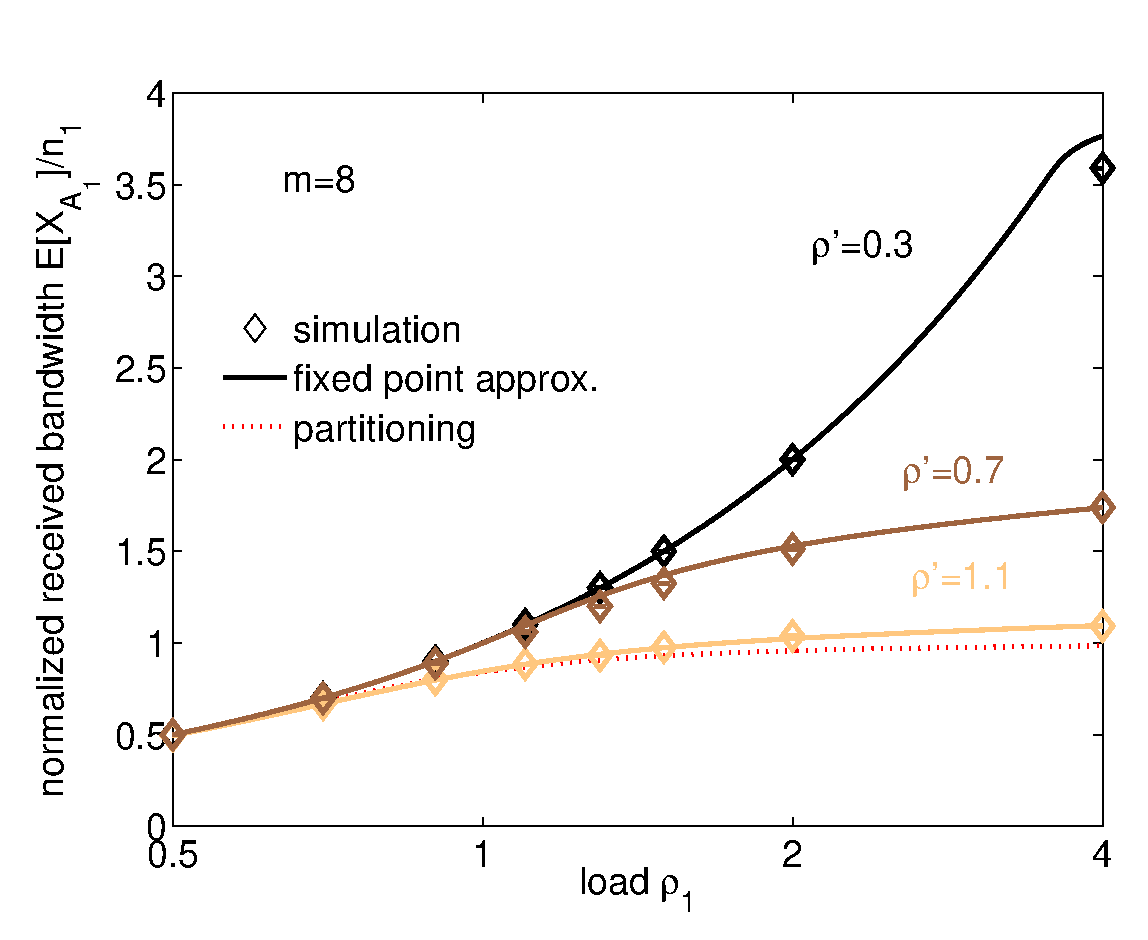
\includegraphics[width=\linewidth]{aggregation/performance_model/figures/fp_bw_m8}
 \caption{Equal load}
 \label{fig:bw_m8}
\end{subfigure}%
\begin{subfigure}{.49\textwidth}
 \centering
 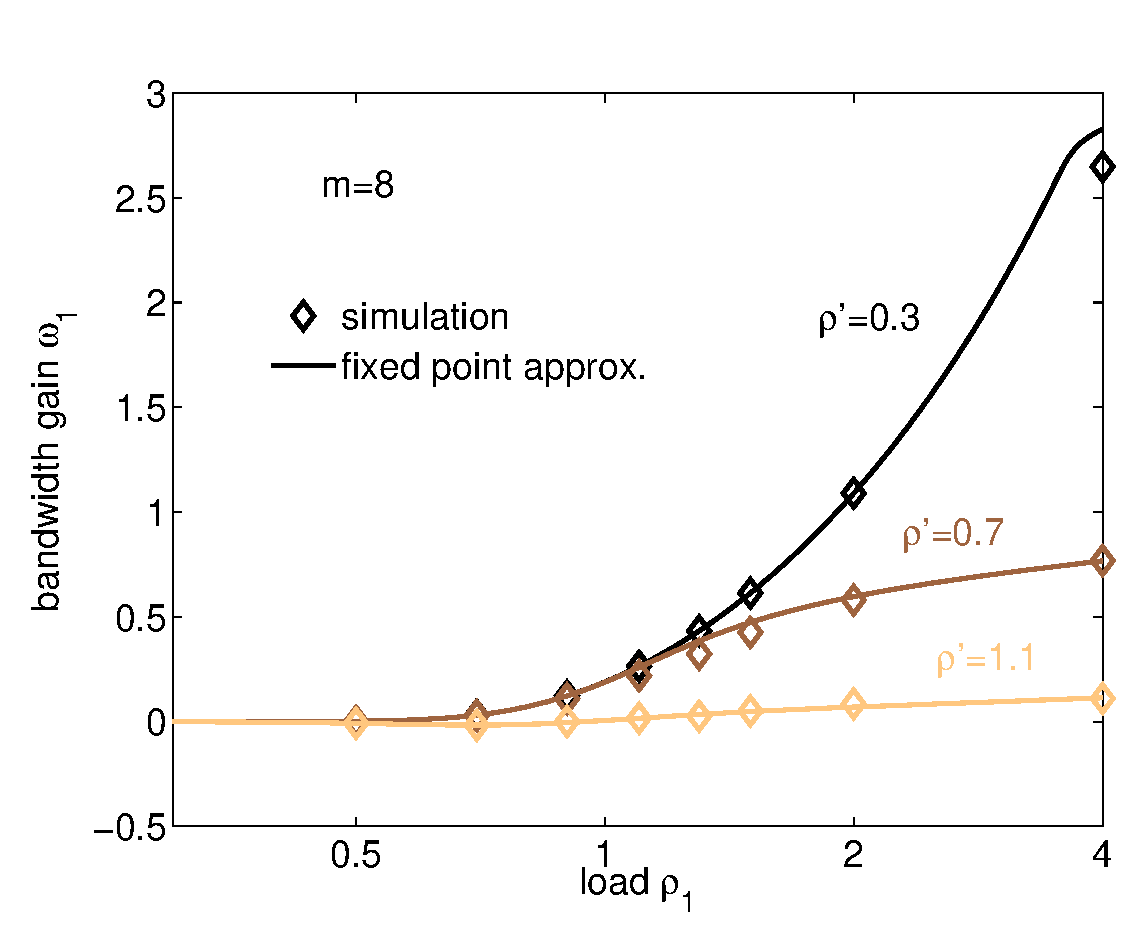
\includegraphics[width=\linewidth]{aggregation/performance_model/figures/fp_bwgain_m8}
 \caption{bandwidth gain $\omega_1$}
 \label{fig:bwgain_m8}
 % 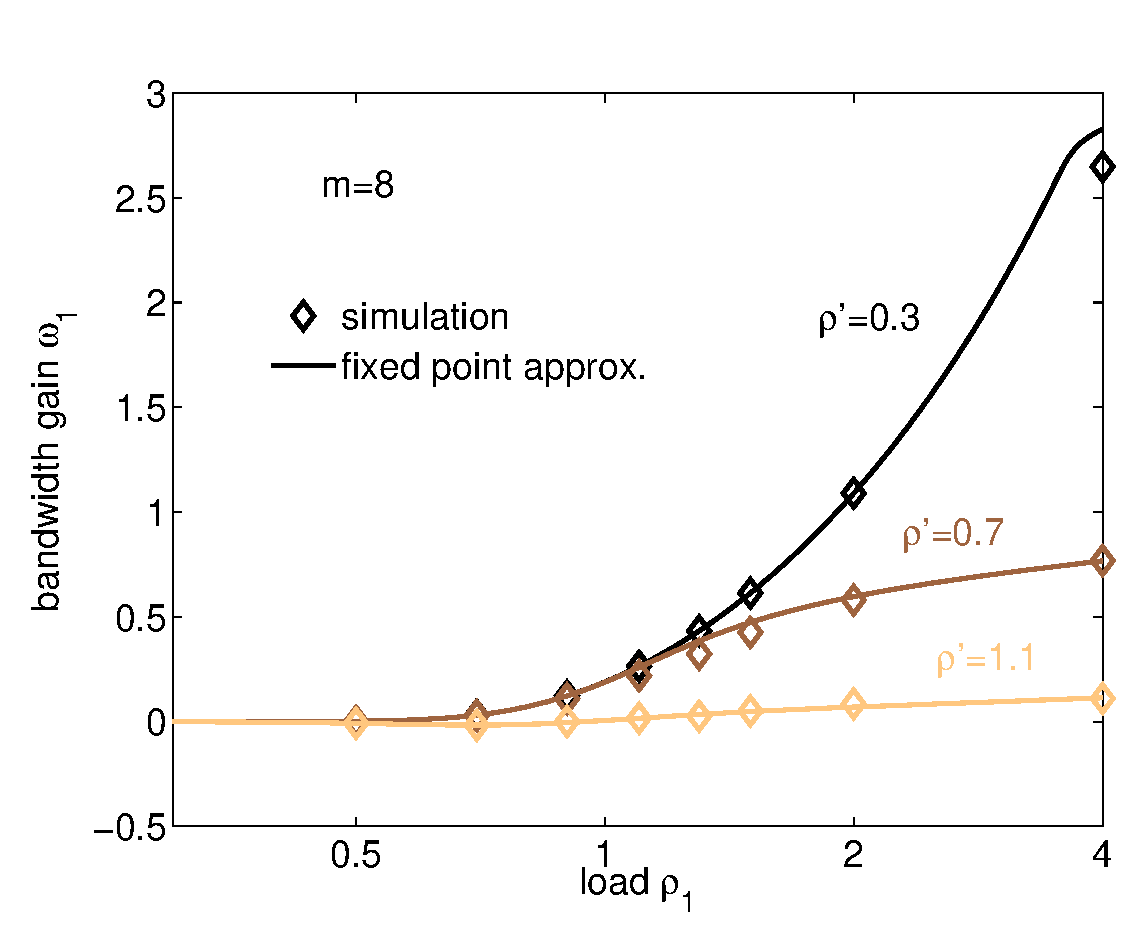
\includegraphics[width=\linewidth]{aggregation/performance_model/figures/fp_bwgain_m8}
 % \caption{bandwidth gain $\omega_1$}
 % \label{fig:bwgain_m8}
\end{subfigure}
\caption{Received bandwidth $E[X_{A_1}]/n_1$ dependent on load of the other links $\rho'$ for $m=8$}
\label{fig:m8}
\end{figure*}

In the following we investigate how the load on the links in the composite system $\rho'$ affects the throughput of the observed system for $m=8$ cooperating systems.
Figure~\ref{fig:bw_m8} shows the normalized received bandwidth of the observed system dependent on the throughput of the links in the composite system $\rho'$.
%The fixed point approximation decently fits the simulation results.
In case of $\rho'=0.3$ a lot of spare bandwidth is available for offloading. If the observed system is overloaded it can use the spare bandwidth and receives almost 400\% of its capacity if its load is 400\%. If the load $\rho'$ on the other links is higher, less bandwidth is available, which limits the received bandwidth. Still, the received bandwidth is above partitioning, although the links in the composite systems are overloaded with $\rho'=1.1$ if the observed system is even more overloaded.
%This can also be seen in the bandwidth gain $\omega_1$ depicted in Figure~\ref{fig:bwgain_m8}, which is positive if the observed system is overloaded with $\rho_1>1$. The bandwidth gain is only marginally negative, if the load on the observed system is low, which is manageable in off-peak periods. In busy periods the observed system benefits a lot by gaining more than 2.5 times more bandwidth if $\rho'=0.3$.

\begin{figure*}[tb]
\centering
\begin{subfigure}{.49\textwidth}
  \centering
  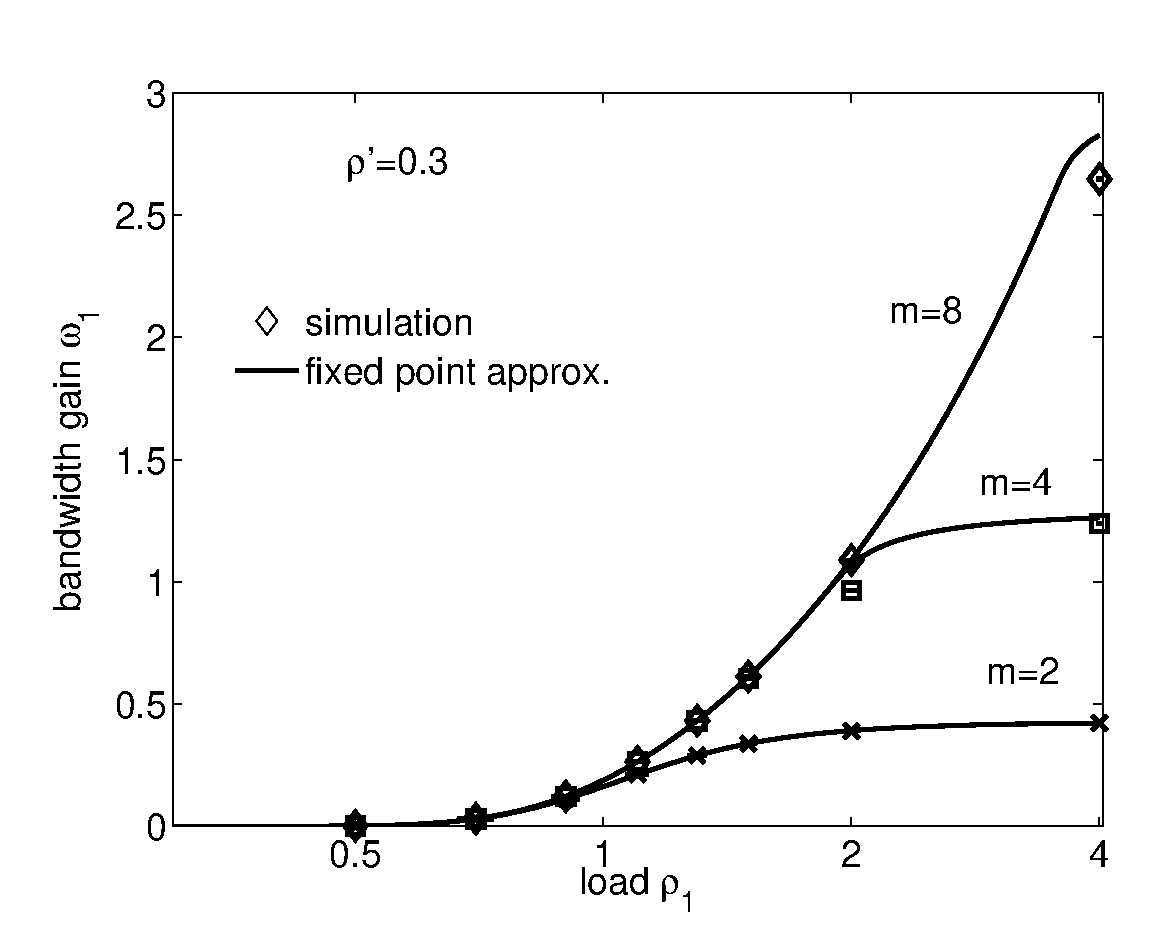
\includegraphics[width=\linewidth]{aggregation/performance_model/figures/fp_bwgain_rho03}
  \caption{Off peak ($\rho'=0.3$)}
  \label{fig:fp_bwgain_rho03}
\end{subfigure}%
\begin{subfigure}{.49\textwidth}
  \centering
  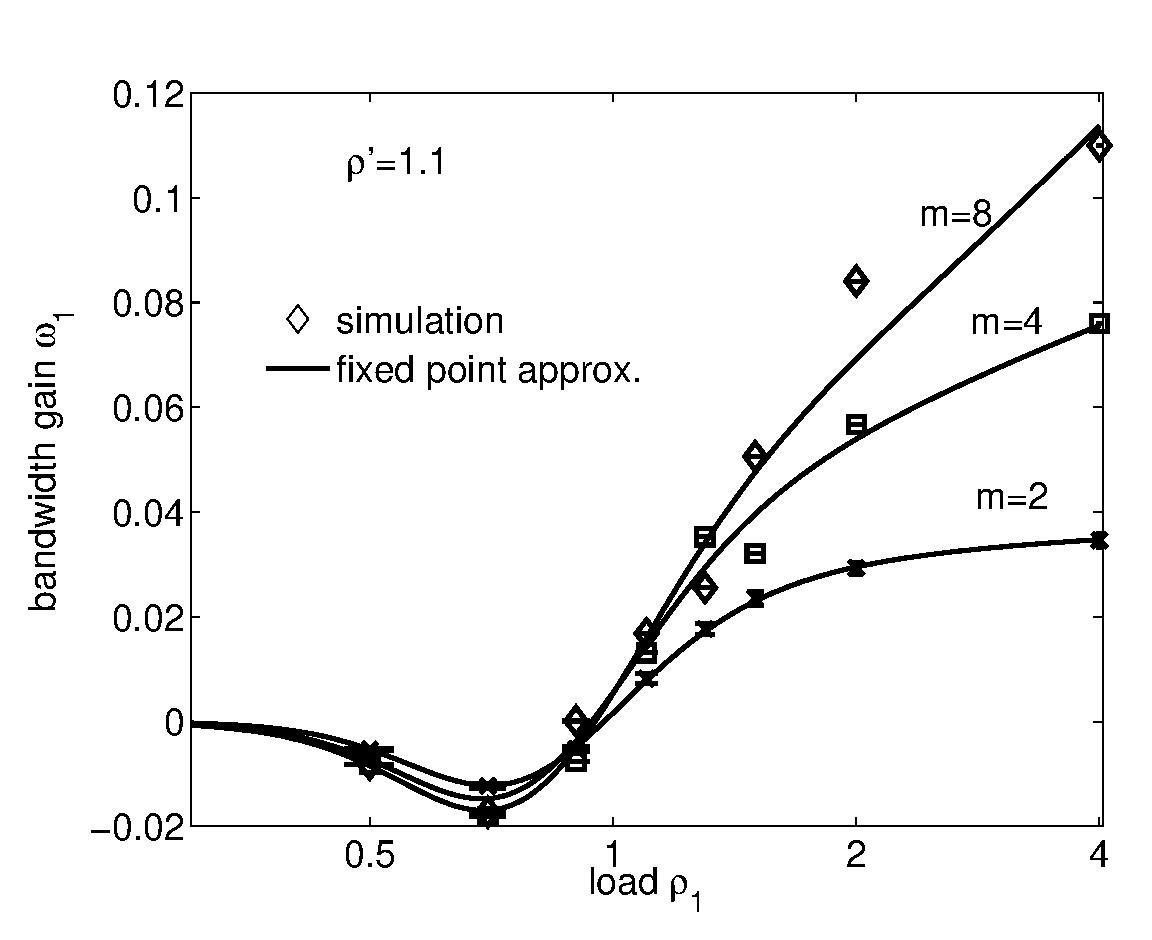
\includegraphics[width=\linewidth]{aggregation/performance_model/figures/fp_bwgain_rho11}
  \caption{Overload ($\rho'=1.1$)}
  \label{fig:fp_bwgain_rho11}
\end{subfigure}
\begin{subfigure}{.49\textwidth}
  \centering
\includegraphics[width=\linewidth]{aggregation/performance_model/figures/fp_bwgain_prio11}
  	\caption{Unfair: ($\alpha_1 \neq \alpha'$)}
  	\label{fig:fp_bwgain_prio11}
\end{subfigure}
\caption{Bandwidth gain dependent on load of the observed system in off peak, overload and unfair operation.}
\label{fig:fp_bwgain}
\end{figure*}

Figure~\ref{fig:fp_bwgain_rho03} shows the bandwidth gain of the observed system $\omega_1$ dependent on the number of cooperating systems $m$ for $\rho'=0.3$.
Hence, in this case there is a high potential to obtain spare bandwidth from the cooperating systems.
%Independent of the number of cooperating systems $m$, the bandwidth gain increases with the load $\rho_1$ on the observed system.
Depending on the number of cooperating systems the bandwidth gain of the observed system is limited.
%Up to a load of $\rho_1=1$, the spare bandwidth of one underutilized system with $\rho'=0.3$ is enough to support the observed system, which achieves the same bandwidth gain as with more cooperating systems.
%The bandwidth gain is equal for 4 and 8 cooperating systems up to a load of $\rho_1=2$.
%For higher loads of the observed system, the bandwidth that can be provided by 4 cooperating links reaches its limit.
%Especially if the number of cooperating systems is high, an overloaded system gains a lot of bandwidth.

Figure~\ref{fig:fp_bwgain_rho11} shows the bandwidth gain of the observed system $\omega_1$ dependent on the number of cooperating systems $m$ for $\rho'=1.1$.
In this case the links in the composite system are overloaded.
This leads to a loss of up to 2\% bandwidth, if the observed system is not overloaded itself.
If the load on the observed system is high, but low enough that it supports other systems, a traffic burst is more likely to block the system, since the overall load is higher than in the partitioning case.
%If the observed system is also overloaded its bandwidth gain increases dependent on the number of cooperating systems.

To conclude, if the load on the other systems is low, an overloaded system can highly profit from their spare bandwidth by gaining multiples of its own bandwidth. The maximum bandwidth gain is limited by the number of cooperating systems $m$.
If the cooperating systems are overloaded, the received bandwidth might be up to 2\% lower in some cases, but this is compensated with multiples of the base level bandwidth in high peak periods.

%\begin{figure}[tb]
%	\centering
% 	\includegraphics[width=0.5\textwidth]{figures/fp_bwgain_prio11}
%  	\caption{Bandwidth gain dependent on the load of the observed system in egoistic ($\alpha_1$=0\%,$\alpha'$=70\%), normal ($\alpha_1$=70\%,$\alpha'$=70\%) and altruistic ($\alpha_1$=70\%,$\alpha'$=0\%) operation.}
%  	\label{fig:fp_bwgain_prio11}
%\end{figure}

To prevent a system from being congested from an overloaded cooperating system, it can be prioritized. One possibility of prioritizing is to decrease the support threshold $\alpha$, so that it still can offload to other systems, but shares less bandwidth fractions to support. Figure~\ref{fig:fp_bwgain_prio11} shows the bandwidth gain of the observed system for three cases. The dotted line shows the blocking probability if observed and other systems have equal support threshold $\alpha_1=\alpha'=70\%$. The solid line shows the case where the observed system is altruistic and keeps its threshold at $\alpha_1=70\%$, but interacts with egoistic cooperating systems with support threshold $\alpha'=0\%$. The dashed line shows the egoistic case where the observed system limits its support threshold to $\alpha_1=0\%$, while the cooperating systems support up to $\alpha'=70\%$. The altruistic system suffers from egoistic cooperating systems by losing up to about 3\% bandwidth while not being able to gain bandwidth in high loads. Compared to that, the bandwidth gain in the egoistic case is never negative.
Hence, if a system is egoistic it always gains more bandwidth. However, the gain compared to normal operation is not high, and if each system would be egoistic no bandwidth can be shared. This would mean completely partitioned systems which would not change the current situation without bandwidth sharing.
On the other hand, if a system is the only one sharing among only free riders, which corresponds to the altruistic case, the situation is not worse, since only about 3\% of the bandwidth are lost.
Thus it is a win-win situation if everybody contributes to the system and shares spare bandwidth.
This provides incentives for systems to contribute.
%However, losing only up to about 3\% bandwidth in the case, where $m-1=7$ egoistic systems with high load ($\rho'=1.1$) are trying to exploit an altruistic system, shows that the mechanism is quite robust against free riders.
%The gain of the egoistic system decreases with the load of the cooperating system.
%Hence, prioritizing is only viable if the cooperating system is highly loaded.

\subsection{Simulation with General Service Times}\label{sec:simgeneral}

To assess the system performance in more general cases we run simulations with different service time distributions.
Figure~\ref{fig:m2_n20_rho2_sim} shows the blocking probability of the reference system dependent on the load of the systems. The mean values with 95\% confidence intervals of 8 simulation runs are plotted for the service time distributions deterministic and hyper-exponential.
The service times in the deterministic process are constant.
In the hyper-exponential process we use two branches with probabilities 10\% and 90\%.
For constant service times the blocking probability does not differ from the analytic model for high system loads. The blocking probability differs slightly from the analytic model for deterministic service times in low system loads, showing higher blocking probabilities if the load on the cooperating system is high. The reason for this has to be investigated and is part of future work. In case of the hyper-exponential distribution the service times are highly variant. Here the system which is highly loaded benefits from lower blocking probabilities compared to the analytic model.

% \begin{figure}[tb]
% 	\centering
% 	\includegraphics[width=0.5\textwidth]{aggregation/performance_model/figures/m2_n20_rho2_sim}
%  	\caption{Blocking probability dependent on the load of reference and cooperating system. Simulation with different service time distributions.}
%  	\label{fig:m2_n20_rho2_sim}
% \end{figure}

\begin{figure*}[tb]
\centering
\begin{subfigure}{.49\textwidth}
 \centering
 \includegraphics[width=\linewidth]{aggregation/performance_model/figures/m2_n20_rho2_sim}
 \caption{Blocking probability}
 \label{fig:m2_n20_rho2_sim}
\end{subfigure}%
\begin{subfigure}{.49\textwidth}
 \centering
 \includegraphics[width=\linewidth]{aggregation/performance_model/figures/bw_n20_rho2_sim}
 \caption{Received bandwidth}
 \label{fig:bw_n20_rho2_sim}
\end{subfigure}
\caption{Blocking probability and received bandwidth dependent on the load of reference and cooperating system. Simulation with different service time distributions.}
\label{fig:n20_rho2_sim}
\end{figure*}

In Figure~\ref{fig:bw_n20_rho2_sim}, which shows the received bandwidth of the reference system dependent on the load, simulation results are plotted for deterministic distributed and highly variant hyper-exponential distributed service times.
For deterministic service times the analytic model fits the simulation results. If the service times are highly variant the reference system receives only slightly more bandwidth than in the model if it is overloaded. Hence, considering the available bandwidth the analytic model can be used to assess the system performance with general service time distributions.

% \begin{figure}[tb]
% 	\centering
% 	\includegraphics[width=0.5\textwidth]{aggregation/performance_model/figures/m2_n20_q1}
%  	\caption{Blocking probability of two queues dependent on load.}
%  	\label{fig:m2_rho2_q1}
% \end{figure}


\section{Backhaul Bandwidth Aggregation in Imbalanced Load}\label{sec:aggregation:imbalanced}

To assess the full potential of the approach, we consider an inner and an outer composite system. Thus, we are able to apply the method to the case of heterogeneous load in \refsec{sec:aggregation:imbalanced:analytical_model}, which allows evaluating the gain in situations where an overloaded system can use spare bandwidth of underutilized links \refsec{sec:aggregation:imbalanced:numerical_examples}.
This further allows us to evaluate the fairness of the system and its robustness against free riders that try to exploit the system by receiving available bandwidth without contributing spare bandwidth to neighboring systems.

%\section{System Dynamics in Fair Operation}\label{sec:aggregation:performance_model:analytical_model}

%\subsubsection*{System Model}\label{sec:network:performance_model:analytical_model:system_model}


\subsection{The Case of Two Systems}\label{sec:aggregation:performance_model:analytical_model:2_systems}

% \begin{figure}[htb!]
% 	\centering
%  	\includegraphics[width=0.66\textwidth]{figures/sysmodel3}
%   	\caption{System model.}
%   	\label{fig:sysmodel}
% \end{figure}


We first consider a scenario with two different Internet access links. %Figure~\ref{fig:sysmodel} shows a schematic view of the model as described above and highlights the most important system characteristics.
In the case of two links, the actual system state can be described by two random variables $X_1$ and $X_2$, which represent the number of occupied bandwidth fractions in the respective access link. As the model components comprise the memoryless property, a two-dimensional Markov process can be analyzed using standard techniques of queueing theory.

With the state probabilities
\begin{equation}
x(i,j) = P(X_1=i, X_2=j),\ 0\leq i\leq n_1, 0\leq j \leq n_2,
\end{equation}
i.e., the probability that $i$ bandwidth fractions are occupied in system 1 and $j$ bandwidth fractions are occupied in system 2, the two-dimensional state transition diagram, presented in Figure~\ref{fig:statetransitions}, can be arranged. Two major areas are visible. In the upper left part and the lower right part (white background), each system operates independently in such way that all arriving requests are served locally by this system. In the top-right and bottom-left parts (shaded in gray), one of the links is in offloading state and the other link is in support state. In these cases, all traffic arriving at the offloading link will be served by the supporting link. Thus, blocking only occurs when the other link cannot help, i.e., in states $\{(n_1,j) : \lfloor\alpha_2 n_2\rfloor \leq j \leq n_2\}$ and $\{(i,n_2) : \lfloor\alpha_1 n_1\rfloor\leq i \leq n_1\}$.

\begin{figure*}[tb]
	\centering
 	\includegraphics[width=1.0\textwidth]{aggregation/performance_model/figures/states}
  	\caption{The state transition diagram.}
  	\label{fig:statetransitions}
\end{figure*}

Having the state probabilities, we calculate the blocking probability $p_{b_i}$ of each system $i$ and the total blocking probability $p_b$, which is the sum of blocking probabilities of each system weighted by the probability that a request arrives at each respective system.

\begin{equation}
p_{b_1} = \sum_{k=\lfloor\alpha_2\cdot n_2\rfloor}^{n_2} x(n_1,k),\quad p_{b_2} = \sum_{k=\lfloor\alpha_1\cdot n_1\rfloor}^{n_1} x(k,n_2)
\end{equation}
\begin{equation}
 p_{b} = \frac{\lambda_1}{\lambda_1+\lambda_2}\cdot p_{b_1}+\frac{\lambda_2}{\lambda_1+\lambda_2}\cdot p_{b_2}
\end{equation}

Since requests can be offloaded from system 1 to system 2 in states $(n_1, k)$ for $k<\lfloor\alpha_2\cdot n_2\rfloor$, the requests are not blocked and the state probabilites are not added to the blocking probability $p_{b_1}$. The same holds for states $(k, n_2)$ with $k<\lfloor\alpha_1\cdot n_1\rfloor$ and $p_{b_2}$.

% The blocking probabilities for each link $p_{b_1}$ and $p_{b_2}$ are calculated by
%
% \begin{equation}
%   p_{b_1} = \sum_{j=\lfloor\alpha_2 n_2\rfloor}^{n_2}x(n_1,j)
% \end{equation}
% and
% \begin{equation}
%   p_{b_2} = \sum_{i=\lfloor\alpha_1 n_1\rfloor}^{n_1}x(i,n_2) \, ,
% \end{equation}
%
% and the total blocking probability $p_b$ is calculated by considering the probability of an arrival at each of the links:
%
% \begin{equation}
%   p_{b} = \frac{\lambda_1}{\lambda_1+\lambda_2} p_{b_1} + \frac{\lambda_2}{\lambda_1+\lambda_2} p_{b_2} \, .
% \end{equation}

\subsection{The Case of Multiple Systems}\label{sec:aggregation:performance_model:analytical_model:m_systems}

The case, in which $m$ Internet access links offload traffic according to the policy defined via the support and offloading thresholds, is more interesting, since much more than two access links can be available in densely populated neighborhoods and since the potential of the approach increases with the number of links available for bandwidth sharing.
We start with assuming that all access links are equal ($n=n_i, \forall i\in\{1,\ldots,m\}$) and face equal loads ($\lambda=\lambda_i, \forall i\in\{1,\ldots,m\}$) and policies ($\alpha = \alpha_i, \beta = \beta_i, \forall i\in\{1,\ldots,m\}$). First, we distinguish one access link, and merge the remaining $m-1$ cooperating access links into a composite system. This reduces the problem of $m$ systems to two systems. Still, the complexity of the composite system prohibits creating and analyzing the two-dimensional state transition diagram as it was done in \cite{burger2016phycom}. Thus, we apply a fixed point approach to analyze this system.%, which is presented in Figure~\ref{fig:composite}.
Therefore, we model an observed system, which will take into account offloading to and supporting the abstract composite system. For simplifying the notation, we define the macro state probabilities $p_1$ (support), $p_2$ (normal), and $p_3$ (offload):

\begin{align}
\begin{split}
p_1 &= \sum x(i),  0 \leq i < \lfloor\alpha\cdot n\rfloor \\
p_2 &= \sum x(i), \lfloor\alpha\cdot n\rfloor\leq i < \lfloor\beta\cdot n\rfloor \\
p_3 &= \sum x(i), \lfloor\beta\cdot n\rfloor \leq i \leq n
\end{split}
\label{eq:macro}
\end{align}

In the support macro state, the arrival rate will be increased by $\lambda_s$, i.e., the arrivals that are offloaded by the composite system. $\lambda_s$ can be computed as shown in Equation~\ref{eq:lambda_s} from the multinomial probability that $j$ of the $m-1$ links in the composite system are in offloading state, and $k$ links in the composite system can support.

\small
\begin{equation}
\lambda_{s} = \sum_{j=1}^{m-1}\sum_{k=0}^{m-1-j} \binom{m-1}{j}\binom{m-j-1}{k}p^j_3 p^k_1 p_2^{m-j-k-1}\frac{j\lambda}{k+1}
\label{eq:lambda_s}
\end{equation}
\normalsize

The arrival rate is decreased by $\lambda_o$ in the offloading macro state when the composite system can support the observed system, i.e., at least one of the $m-1$ systems is in support macro state.

\begin{equation}
\lambda_{o} = (1-(1-p_1)^{m-1})\lambda
\end{equation}

This gives new steady state equations for the observed system as described in Equation~\ref{eq:iteration}. As all access links have equal load, and thus, show a homogeneous behavior, not only the state probabilities of the observed system, but also of the $m-1$ systems in the composite system are influenced. Thus, the state probabilities of all $m$ links can be obtained by computing the state probabilities of the observed system. Therefore, we initialize the observed system with equal state probabilities. Then, we iterate the offloading and support and normalize the state probabilities  until a fixed point is reached.

\begin{align}
\begin{split}
&x(i)=
\begin{cases}
\frac{x(i-1)(\lambda+\lambda_s)}{i\cdot\mu}, &0\leq i < \lfloor\alpha\cdot n\rfloor \\
\frac{x(i-1)\lambda}{i\cdot\mu}, &\lfloor\alpha\cdot n\rfloor\leq i < \lfloor\beta\cdot n\rfloor \\
\frac{x(i-1)(\lambda-\lambda_o)}{i\cdot\mu}, &\lfloor\beta\cdot n\rfloor \leq i \leq n \\
\end{cases}\\
&\sum_{i=0}^n x(i) = 1
\end{split}
\label{eq:iteration}
\end{align}

For our modeled bandwidth aggregation system with $m$ Internet access links, we consider the blocking probability $p_{b} = x(n)\cdot (1-p_1)^{m-1}$ of a link, which is calculated by the probability that a request arrives when the link is fully loaded (i.e., in state $n$) and none of the $m-1$ other links can support.

Moreover, we take a look at the received bandwidth at each access link $E[X_{A_i}]$. Thereby, $X_{A_i}$ is a random variable for the number of bandwidth fractions (in all systems), which are occupied by arrivals from system $i$. It is obvious that $E[X_{A_i}] = E_0[X_i]$ for the partitioned system. In case of offloading between $m$ equal links, $E[X_{A_i}]= \frac{\lambda}{\mu}\cdot (1-p_{b})$ is equal for all links and can be calculated from the mean total number of occupied bandwidth fractions by taking into account the share of accepted requests.
Finally, we also quantify the percentage of bandwidth gain for each system as
\begin{equation}
\omega_i = \frac{E[X_{A_i}]-E_0[X_i]}{E_0[X_i]}\, .
\end{equation}

\subsection{Numerical Examples and Implications on Fairness}\label{sec:aggregation:imbalanced:numerical_examples}

The cooperating system can benefit if the load is heterogeneously distributed among the systems, such that a system which is currently busy can offload to an idle system.
%To investigate the performance in heterogeneous load conditions we calculate the blocking probability $p_{b_1}$ of the observed system dependent on its load $\rho_1$ and the load on the links in the composite system $\rho' = \rho_i, i\in\{2,\ldots,m\}$.

In order to assess the potential of bandwidth aggregation of $m$ systems in heterogeneous load conditions, we study the load of the observed system $\rho_1$ and set the load of the other $m-1$ systems to the same value $\rho'$, i.e., $\rho_i=\rho',\forall i\in\{2,\dotsc,m\}$.
%As performance metric we consider the normalized received bandwidth of the observed system $E[X_{A_1}]/n_1$ and the bandwidth gain of the observed system $\omega_1$. We first investigate the impact of the impact of $\rho'$, then we investigate the number of cooperating systems $m$ for a fixed load $\rho'$.

\begin{figure*}[tb]
\centering
\begin{subfigure}{.49\textwidth}
 \centering
 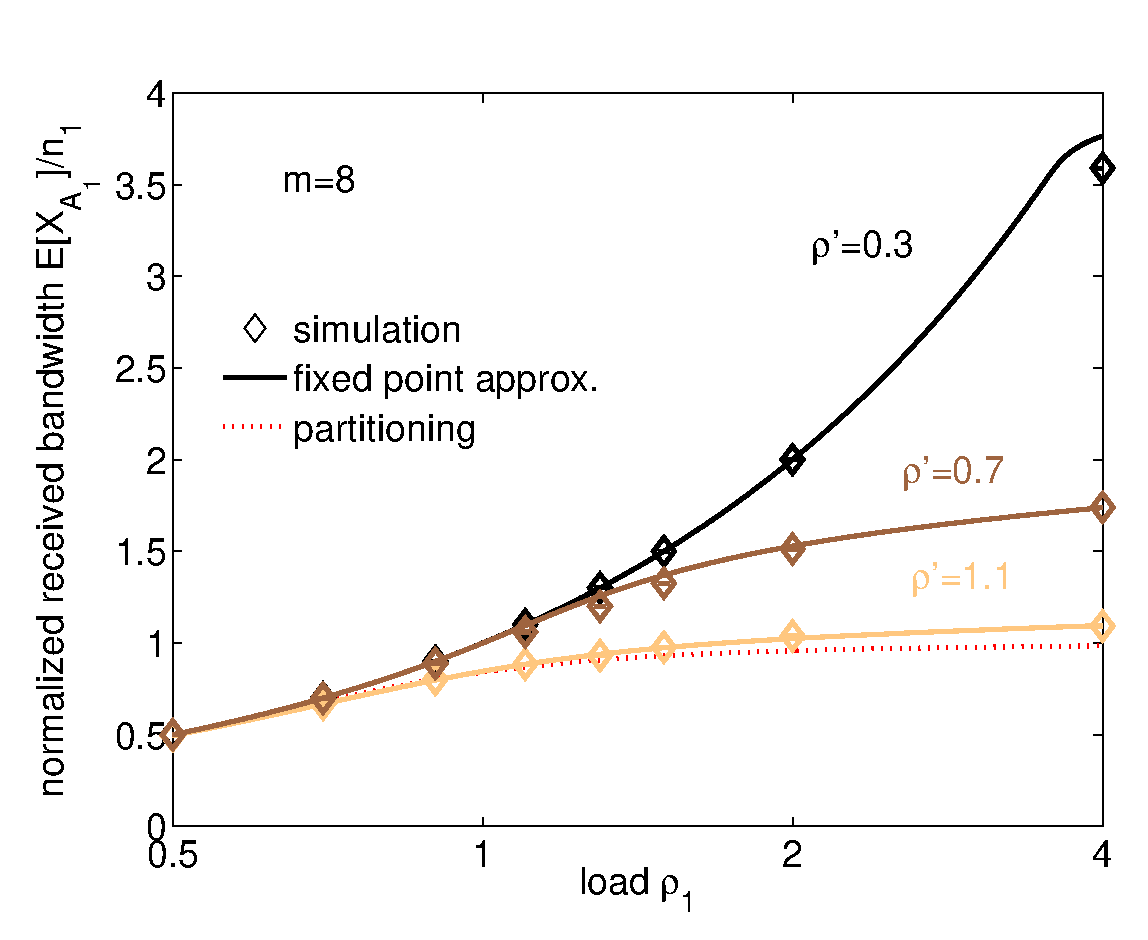
\includegraphics[width=\linewidth]{aggregation/performance_model/figures/fp_bw_m8}
 \caption{Equal load}
 \label{fig:bw_m8}
\end{subfigure}%
\begin{subfigure}{.49\textwidth}
 \centering
 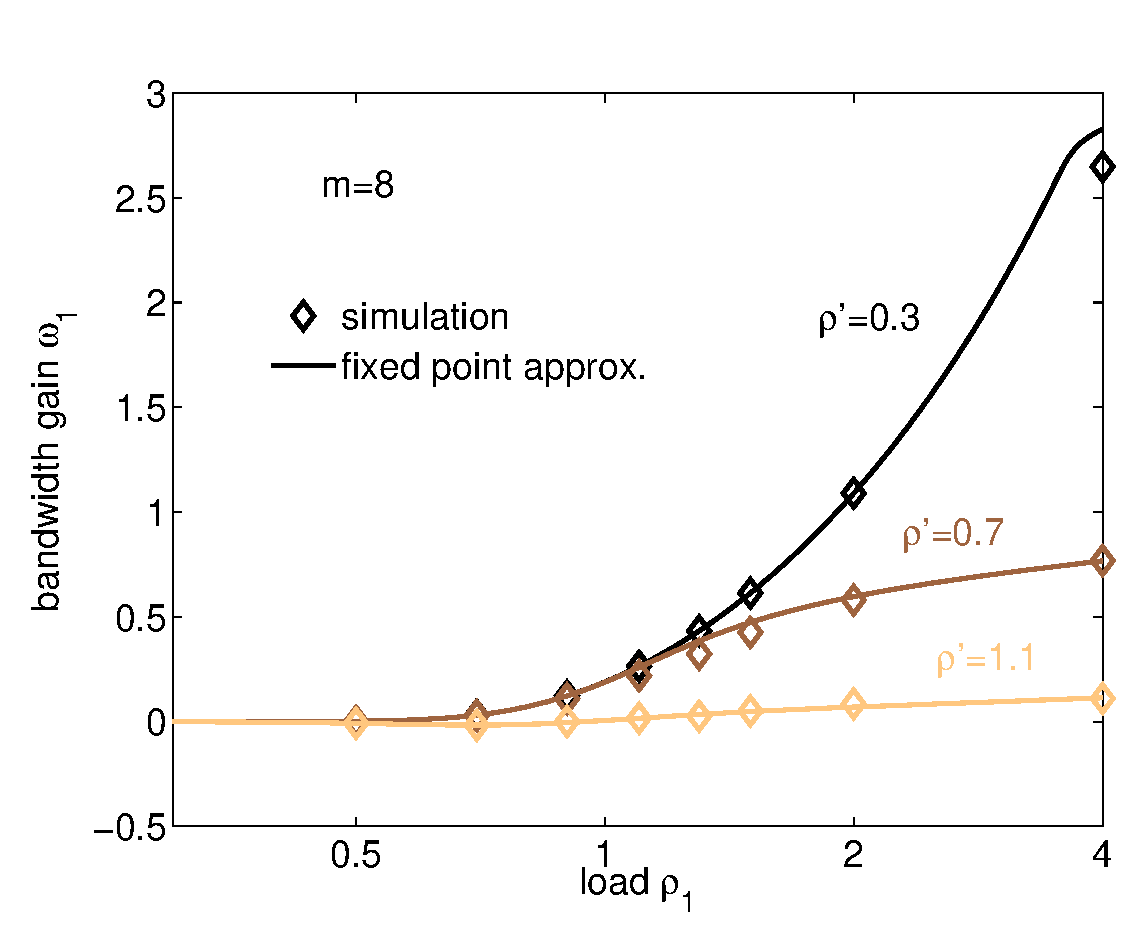
\includegraphics[width=\linewidth]{aggregation/performance_model/figures/fp_bwgain_m8}
 \caption{bandwidth gain $\omega_1$}
 \label{fig:bwgain_m8}
 % 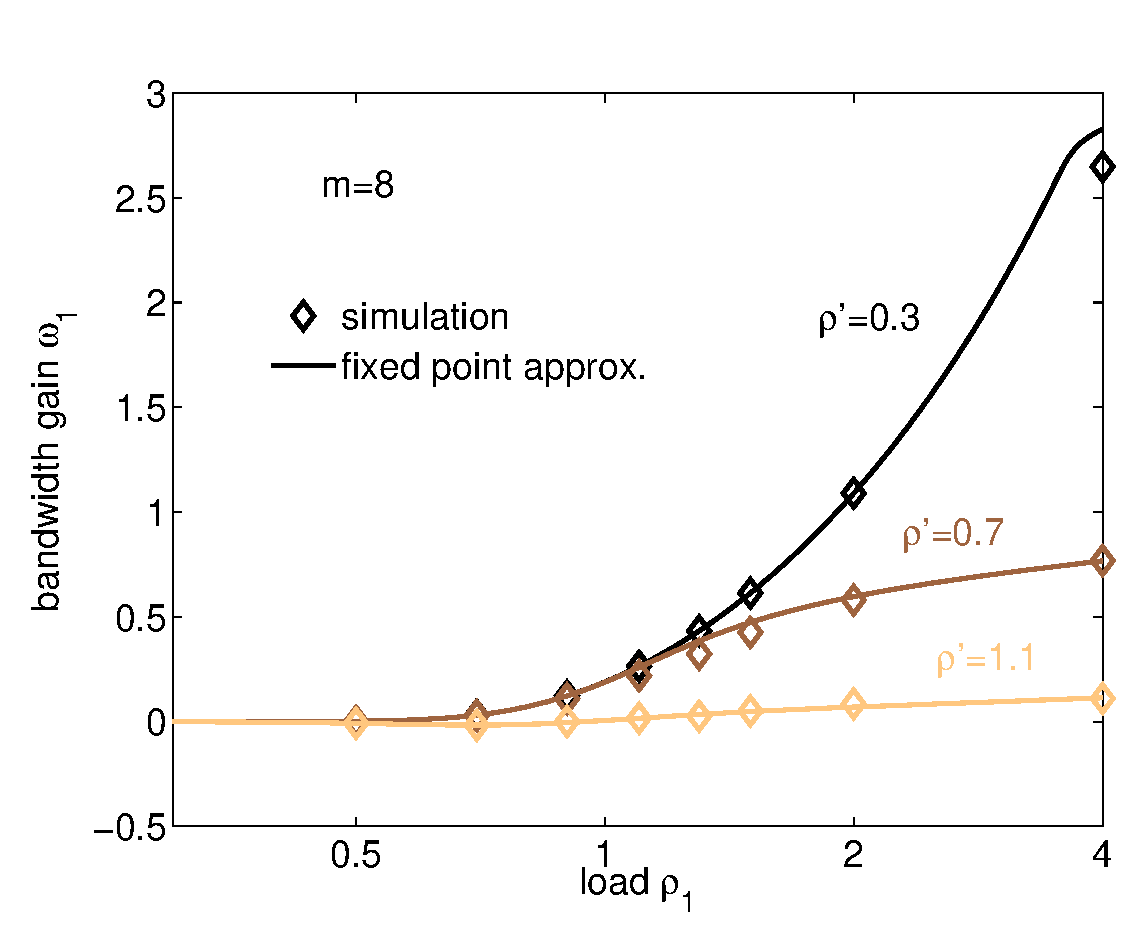
\includegraphics[width=\linewidth]{aggregation/performance_model/figures/fp_bwgain_m8}
 % \caption{bandwidth gain $\omega_1$}
 % \label{fig:bwgain_m8}
\end{subfigure}
\caption{Received bandwidth $E[X_{A_1}]/n_1$ dependent on load of the other links $\rho'$ for $m=8$}
\label{fig:m8}
\end{figure*}

In the following we investigate how the load on the links in the composite system $\rho'$ affects the throughput of the observed system for $m=8$ cooperating systems.
Figure~\ref{fig:bw_m8} shows the normalized received bandwidth of the observed system dependent on the throughput of the links in the composite system $\rho'$.
%The fixed point approximation decently fits the simulation results.
In case of $\rho'=0.3$ a lot of spare bandwidth is available for offloading. If the observed system is overloaded it can use the spare bandwidth and receives almost 400\% of its capacity if its load is 400\%. If the load $\rho'$ on the other links is higher, less bandwidth is available, which limits the received bandwidth. Still, the received bandwidth is above partitioning, although the links in the composite systems are overloaded with $\rho'=1.1$ if the observed system is even more overloaded.
%This can also be seen in the bandwidth gain $\omega_1$ depicted in Figure~\ref{fig:bwgain_m8}, which is positive if the observed system is overloaded with $\rho_1>1$. The bandwidth gain is only marginally negative, if the load on the observed system is low, which is manageable in off-peak periods. In busy periods the observed system benefits a lot by gaining more than 2.5 times more bandwidth if $\rho'=0.3$.

\begin{figure*}[tb]
\centering
\begin{subfigure}{.49\textwidth}
  \centering
  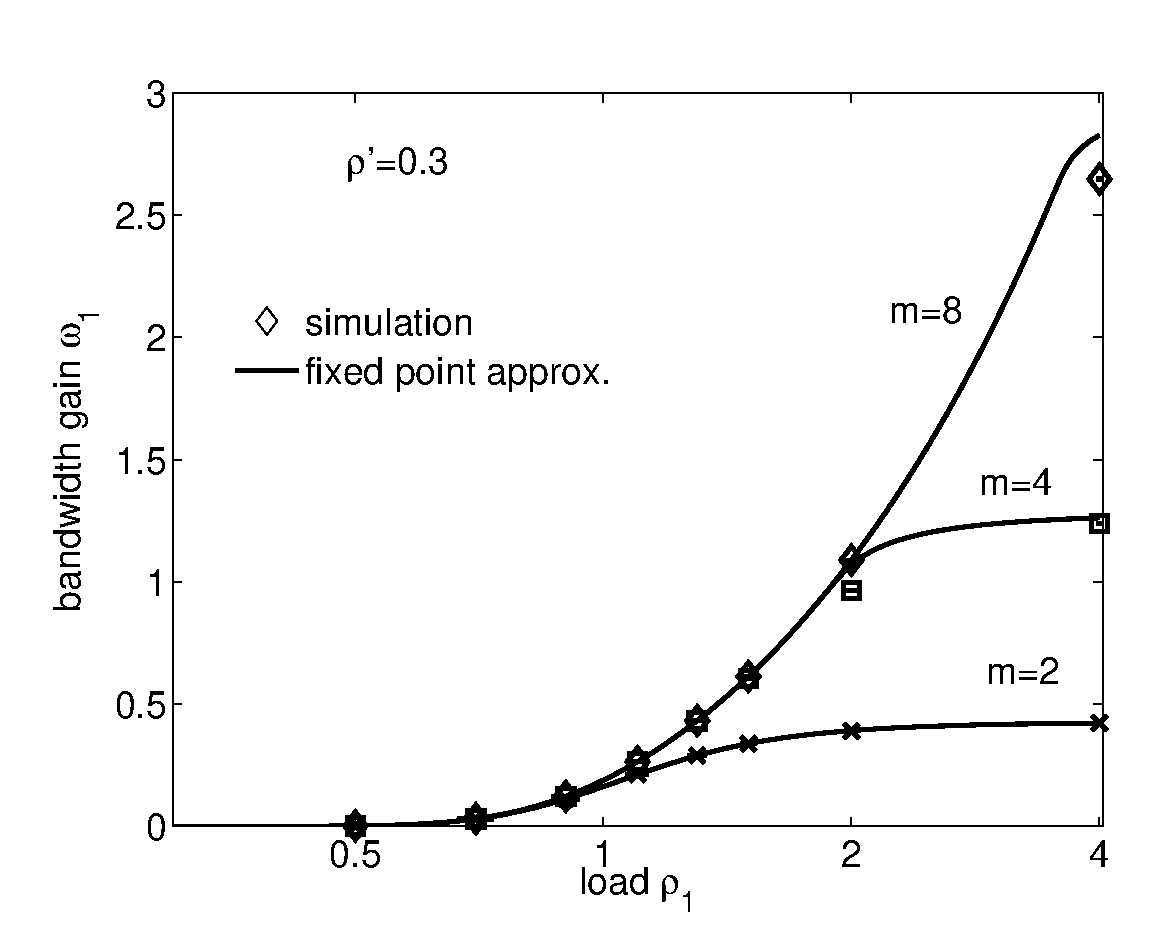
\includegraphics[width=\linewidth]{aggregation/performance_model/figures/fp_bwgain_rho03}
  \caption{Off peak ($\rho'=0.3$)}
  \label{fig:fp_bwgain_rho03}
\end{subfigure}%
\begin{subfigure}{.49\textwidth}
  \centering
  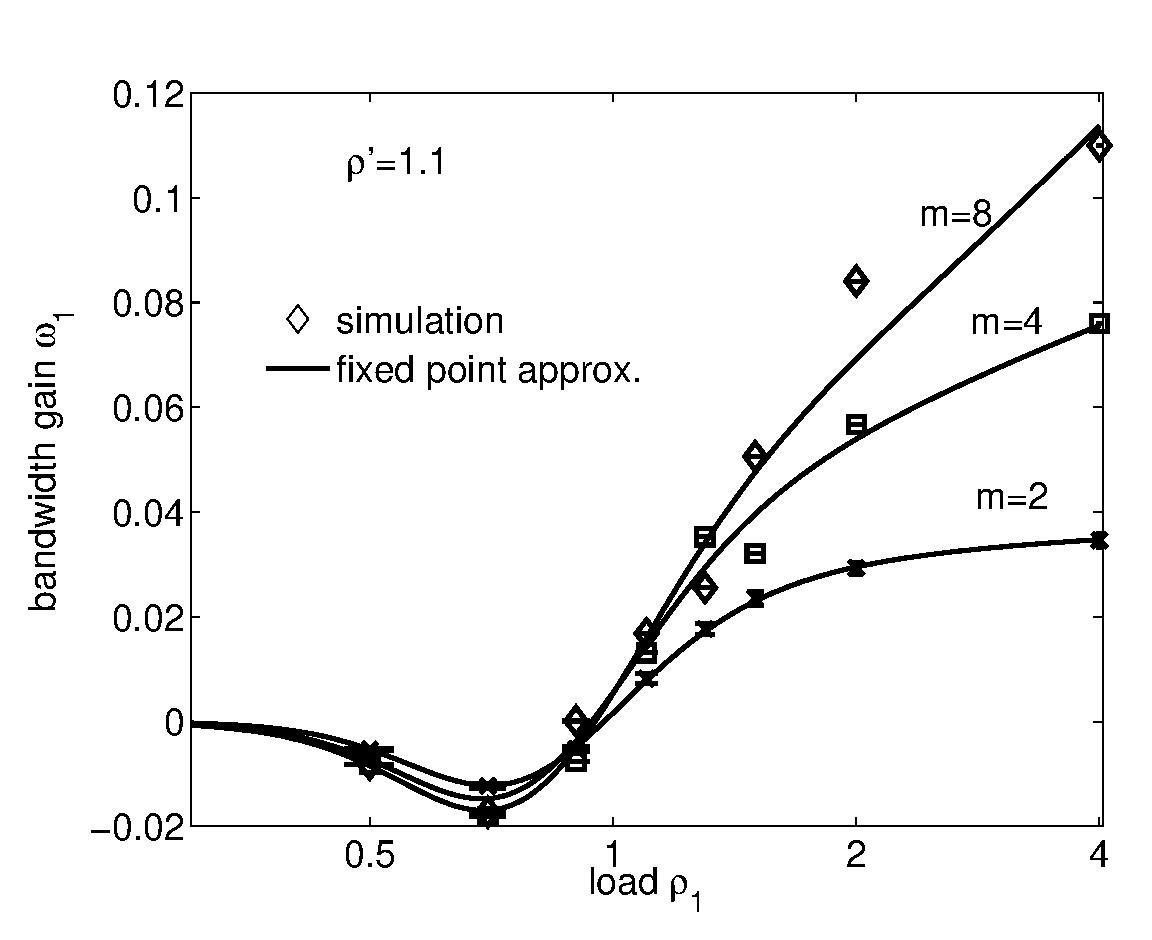
\includegraphics[width=\linewidth]{aggregation/performance_model/figures/fp_bwgain_rho11}
  \caption{Overload ($\rho'=1.1$)}
  \label{fig:fp_bwgain_rho11}
\end{subfigure}
\begin{subfigure}{.49\textwidth}
  \centering
\includegraphics[width=\linewidth]{aggregation/performance_model/figures/fp_bwgain_prio11}
  	\caption{Unfair: ($\alpha_1 \neq \alpha'$)}
  	\label{fig:fp_bwgain_prio11}
\end{subfigure}
\caption{Bandwidth gain dependent on load of the observed system in off peak, overload and unfair operation.}
\label{fig:fp_bwgain}
\end{figure*}

Figure~\ref{fig:fp_bwgain_rho03} shows the bandwidth gain of the observed system $\omega_1$ dependent on the number of cooperating systems $m$ for $\rho'=0.3$.
Hence, in this case there is a high potential to obtain spare bandwidth from the cooperating systems.
%Independent of the number of cooperating systems $m$, the bandwidth gain increases with the load $\rho_1$ on the observed system.
Depending on the number of cooperating systems the bandwidth gain of the observed system is limited.
%Up to a load of $\rho_1=1$, the spare bandwidth of one underutilized system with $\rho'=0.3$ is enough to support the observed system, which achieves the same bandwidth gain as with more cooperating systems.
%The bandwidth gain is equal for 4 and 8 cooperating systems up to a load of $\rho_1=2$.
%For higher loads of the observed system, the bandwidth that can be provided by 4 cooperating links reaches its limit.
%Especially if the number of cooperating systems is high, an overloaded system gains a lot of bandwidth.

Figure~\ref{fig:fp_bwgain_rho11} shows the bandwidth gain of the observed system $\omega_1$ dependent on the number of cooperating systems $m$ for $\rho'=1.1$.
In this case the links in the composite system are overloaded.
This leads to a loss of up to 2\% bandwidth, if the observed system is not overloaded itself.
If the load on the observed system is high, but low enough that it supports other systems, a traffic burst is more likely to block the system, since the overall load is higher than in the partitioning case.
%If the observed system is also overloaded its bandwidth gain increases dependent on the number of cooperating systems.

To conclude, if the load on the other systems is low, an overloaded system can highly profit from their spare bandwidth by gaining multiples of its own bandwidth. The maximum bandwidth gain is limited by the number of cooperating systems $m$.
If the cooperating systems are overloaded, the received bandwidth might be up to 2\% lower in some cases, but this is compensated with multiples of the base level bandwidth in high peak periods.

%\begin{figure}[tb]
%	\centering
% 	\includegraphics[width=0.5\textwidth]{figures/fp_bwgain_prio11}
%  	\caption{Bandwidth gain dependent on the load of the observed system in egoistic ($\alpha_1$=0\%,$\alpha'$=70\%), normal ($\alpha_1$=70\%,$\alpha'$=70\%) and altruistic ($\alpha_1$=70\%,$\alpha'$=0\%) operation.}
%  	\label{fig:fp_bwgain_prio11}
%\end{figure}

To prevent a system from being congested from an overloaded cooperating system, it can be prioritized. One possibility of prioritizing is to decrease the support threshold $\alpha$, so that it still can offload to other systems, but shares less bandwidth fractions to support. Figure~\ref{fig:fp_bwgain_prio11} shows the bandwidth gain of the observed system for three cases. The dotted line shows the blocking probability if observed and other systems have equal support threshold $\alpha_1=\alpha'=70\%$. The solid line shows the case where the observed system is altruistic and keeps its threshold at $\alpha_1=70\%$, but interacts with egoistic cooperating systems with support threshold $\alpha'=0\%$. The dashed line shows the egoistic case where the observed system limits its support threshold to $\alpha_1=0\%$, while the cooperating systems support up to $\alpha'=70\%$. The altruistic system suffers from egoistic cooperating systems by losing up to about 3\% bandwidth while not being able to gain bandwidth in high loads. Compared to that, the bandwidth gain in the egoistic case is never negative.
Hence, if a system is egoistic it always gains more bandwidth. However, the gain compared to normal operation is not high, and if each system would be egoistic no bandwidth can be shared. This would mean completely partitioned systems which would not change the current situation without bandwidth sharing.
On the other hand, if a system is the only one sharing among only free riders, which corresponds to the altruistic case, the situation is not worse, since only about 3\% of the bandwidth are lost.
Thus it is a win-win situation if everybody contributes to the system and shares spare bandwidth.
This provides incentives for systems to contribute.
%However, losing only up to about 3\% bandwidth in the case, where $m-1=7$ egoistic systems with high load ($\rho'=1.1$) are trying to exploit an altruistic system, shows that the mechanism is quite robust against free riders.
%The gain of the egoistic system decreases with the load of the cooperating system.
%Hence, prioritizing is only viable if the cooperating system is highly loaded.

\subsection{Simulation with General Service Times}\label{sec:simgeneral}

To assess the system performance in more general cases we run simulations with different service time distributions.
Figure~\ref{fig:m2_n20_rho2_sim} shows the blocking probability of the reference system dependent on the load of the systems. The mean values with 95\% confidence intervals of 8 simulation runs are plotted for the service time distributions deterministic and hyper-exponential.
The service times in the deterministic process are constant.
In the hyper-exponential process we use two branches with probabilities 10\% and 90\%.
For constant service times the blocking probability does not differ from the analytic model for high system loads. The blocking probability differs slightly from the analytic model for deterministic service times in low system loads, showing higher blocking probabilities if the load on the cooperating system is high. The reason for this has to be investigated and is part of future work. In case of the hyper-exponential distribution the service times are highly variant. Here the system which is highly loaded benefits from lower blocking probabilities compared to the analytic model.

% \begin{figure}[tb]
% 	\centering
% 	\includegraphics[width=0.5\textwidth]{aggregation/performance_model/figures/m2_n20_rho2_sim}
%  	\caption{Blocking probability dependent on the load of reference and cooperating system. Simulation with different service time distributions.}
%  	\label{fig:m2_n20_rho2_sim}
% \end{figure}

\begin{figure*}[tb]
\centering
\begin{subfigure}{.49\textwidth}
 \centering
 \includegraphics[width=\linewidth]{aggregation/performance_model/figures/m2_n20_rho2_sim}
 \caption{Blocking probability}
 \label{fig:m2_n20_rho2_sim}
\end{subfigure}%
\begin{subfigure}{.49\textwidth}
 \centering
 \includegraphics[width=\linewidth]{aggregation/performance_model/figures/bw_n20_rho2_sim}
 \caption{Received bandwidth}
 \label{fig:bw_n20_rho2_sim}
\end{subfigure}
\caption{Blocking probability and received bandwidth dependent on the load of reference and cooperating system. Simulation with different service time distributions.}
\label{fig:n20_rho2_sim}
\end{figure*}

In Figure~\ref{fig:bw_n20_rho2_sim}, which shows the received bandwidth of the reference system dependent on the load, simulation results are plotted for deterministic distributed and highly variant hyper-exponential distributed service times.
For deterministic service times the analytic model fits the simulation results. If the service times are highly variant the reference system receives only slightly more bandwidth than in the model if it is overloaded. Hence, considering the available bandwidth the analytic model can be used to assess the system performance with general service time distributions.

% \begin{figure}[tb]
% 	\centering
% 	\includegraphics[width=0.5\textwidth]{aggregation/performance_model/figures/m2_n20_q1}
%  	\caption{Blocking probability of two queues dependent on load.}
%  	\label{fig:m2_rho2_q1}
% \end{figure}


\section{Lessons Learned}\label{sec:aslevel:lessons_learned}
In this chapter we characterize content delivery networks on autonomous systems level. %by evaluating measurements of the most common content delivery principles P2P and CDN.
For that purpose we summarize related work and use measurements conducted on the distributed platform PlanetLab and a crowdsourcing platform.
To assess the potential of content delivery approaches that use local resources, e.g., on home routers, we determine the number of active IP-addresses from the Internet Census dataset.

%P2P -> CDN
%to accurately model content delivery networks ... is described.
%While ... we find three major outcomes.
First, we provide a comprehensive overview on content delivery network concepts and their evolution. We briefly describe the structure of the YouTube CDN and describe the concept of the next generation of hierarchical CDNs, which use local resources to support content delivery.
In order assess the number of local resources available in each AS, we analyze the Internet Census Dataset to derive the distribution of IP-addresses on ASs.
To this end, we use a mapping of IP-addresses to autonomous system numbers.
we find that the distribution of IP-addresses is highly heterogeneous showing that 30\% of the active IPs belong to the 10 largest autonomous systems.
This means that the potential of approaches that use resources on home routers highly depend on the ISP network.

Second, we propose the usage of crowdsourcing platforms for distributed network measurements to increase the coverage of vantage points.
We evaluate the capability to discover global networks by comparing the coverage of video server detected, using a crowdsourcing platform as opposed to using the PlanetLab platform.
To this end, we use exemplary measurements of the global video CDN YouTube, conducted in both the PlanetLab platform as well as the crowdsourcing platform Microworkers.
Our results show that the vantage points of the concurring measurement platforms have very different characteristics.
We show that the distribution of vantage points has high impact on the capability of measuring a global content distribution network.
The capability of PlanetLab to measure a global CDNs is rather low, since 80\% of requests are directed to the United States.
Our results confirm that the coverage of vantage points is increased by crowdsourcing.
Using the crowdsourcing platform we obtain a diverse set of vantage points that reveals more than twice as many autonomous systems deploying video servers than the widely used PlanetLab platform.
%Part of future work is to determine if the coverage of vantage points can be even further increased by targeting workers from specific locations to get representative measurement points for all parts of the world.

Finally, we investigate where in the Internet BitTorrent traffic is located and which ISPs benefit from its optimization. To this end, we use measurements of live BitTorrent swarms to derive the location of BitTorrent peers and data provided by Caida.org in order to calculate the actual AS path between any two peers.
Our results show that the traffic optimization potential depends heavily on the type of ISP. Different ISPs will pursue different strategies to increase revenues.
Our results confirm that selecting peers based on their locality has a high potential to shorten AS paths between peers and to optimize the overlay network. In the observed BitTorrent swarms twice as much traffic can be kept intra-AS using locality peer selection. Thus, the inter-AS traffic is almost reduced by \unit[50]{\%} in \tier and in large ISPs.
%If ...
%This would for example allow ..

Based on the results obtained in this chapter, we develop models that describe the characteristics of CDNs and the number of active subscribers in ISP networks.
The models allow us to analyze the performance of traffic management mechanisms in realistic scenarios.
%Upper bounds / potential of p2p cdn approach.
%Including the application providers as stakeholders and considering their key performance indicators requires new models but also allows us to better understand the impact of mechanisms implemented in applications.
%Key performance indicators of application providers sometimes overlap with those relevant to users, as application providers try to improve the experience of users in order to reduce churn.

%Highlighted by both, the P2P approach and the CDN approach the distribution of peers on autonomous systems and the popularity of content is highly heterogeneous.
%Dynamics (orange paper)
%While general traffic management mechanisms intent to optimize the cdn
%this only increases the efficiency of the ISP cache, which may cause suboptimal results if the popularity of videos large variance.
%Thus, we suggest to  tradeoffs, within reason, to the user.
%This approach could be seen as extending the \emph{Economic Traffic Management} approach to the user.

